\documentclass{article}
\title{COMP4211 Machine Learning PA1}
\author{T Yeung \\ scyeungaf@connect.ust.hk}
\usepackage{float}
\usepackage{graphicx}
\usepackage{microtype}
\begin{document}
\maketitle
\begin{description}
	\section*{Part 1: Data Exploration and Preparation}
	\item \textbf{[Q1] Dataset Overview}.
	\begin{itemize}
		\item \textbf{Size of the Dataset:} There are $31$ feature columns in the dataset and $3539$ instances. There are $2$ target columns at the end.
		\item \textbf{Feature Types}: The following are identified as numerical features (total=17):
				[C6, C14, C16, C17, C18, C19, C20, C21,
				C22, C23, C24, C25, C26, C27, C28, C29, C30]

				The following are identified as categorical variables (total=14): [C0, C1, C2, C3, C4, C5, C7, C8,
				C9, C10, C11, C12, C13, C15]
	\end{itemize}
	\item \textbf{[Q2] Missing Values}
		\begin{itemize}
			\item \textbf{Identifcation: } The table illustrates the proportion of missing values in the dataset. (features not included do not have missing values)
				\begin{center}
					\begin{tabular}{|c|c|}
						\hline
						features & proportion of missing values \\
						\hline
						C0   &  0.008194 \\
						C4   &  0.013846 \\
						C5   &  0.030517 \\
						C8   &  0.023170 \\
						C9   &  0.040124 \\
						C11  &  0.044645 \\
						C12  &  0.048036 \\
						C13  &  0.033908 \\
						C15  &  0.038994 \\
						C17  &  0.041820 \\
						C20  &  0.048319 \\
						C22  &  0.004521 \\
						C23  &  0.007912 \\
						C25  &  0.040689 \\
						C29  &  0.045211  \\
						\hline
					\end{tabular}
				\end{center}
			\item \textbf{Potential Impact}: Depending on how missing values are handled, it might affect analysis and model performance in different ways. Usually we do imputation on missing values, but this may distort the relationship between variables, leading to a biased model that has a lower accuracy.
		\end{itemize}
	\item \textbf{[Q3] Feature Distribution}
		\begin{itemize}
			\item \textbf{Numerical Features}
			The following are identified as discrete features (total=11)"
			[C14, C16, C17, C18, C19, C21, C22, C23, C24, C25, C27].

			The following are identified as continuous features (total=7)
			[C6, C20, C26, C28, C29, C30]

			The distribution of the first 3 numerical features (C6, C14, C16) are described below:
			\begin{center}
				\begin{tabular}{|c|c|c|c|c|}
					\hline
					& mean & median & range & variance \\
					\hline
					C6 & 66.3 & 66.5 & 47.5 to 95.0 & 43.8 \\
					C14 & 23.2 & 20.0 & 17 to 70 & 55.2 \\
					C16 & 0.68 & 0.0 & 0 to 20 & 5.17 \\
					\hline
				\end{tabular}
			\end{center}
			and the corresponding box plot:
			\begin{figure}[H]
				\centering
				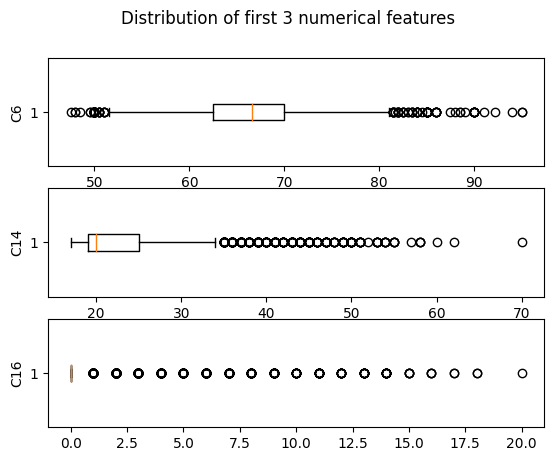
\includegraphics[width=0.8\textwidth]{figures/q3_numerical_distribution.png}
				\caption{Distribution of the first 3 numerical features}
				\label{q3a}
			\end{figure}
			\item \textbf{Categorical Features}
				The following are identified as binary features: [C4, C8, C9, C10, C11, C12, C13, C15] (total=8).

				The following are identified as ordinal features: [C1, C2, C5] (total=3). This is because C1 contains values like "1st phase", "2nd phase", which contains some kind of order. C2 contains values like "first choice", "second choice", possibly indicating preferences. C5 contains values relevant to education status which implies certain hierarchy.

				The following are identified as nominal features: [C0, C3, C4, C7, C8, C9, C10, C11, C12, C13, C15] (total=11). These features do not imply hierarchy in them.

				The following tables present the categorical count of the first 3 categorical features (C0, C1, C2)

				Categories count for C0:
				\begin{center}
					\begin{tabular}{|c|c|}
						\hline
						value & count \\
						\hline
						single               &3115 \\
						married              & 296 \\
						divorced             &  75 \\
						facto union          &  18 \\
						legally separated    &   3 \\
						widower              &   3 \\
						\hline
					\end{tabular}
				\end{center}

				Categories count for C1:
				\begin{center}
					\begin{tabular}{|c|c|}
						\hline
						value & count \\
						\hline
						1st phase - general contingent                        & 1351 \\
						2nd phase - general contingent                         &708 \\
						Over 23 years old                                      &630 \\
						Change of course                                       &253 \\
						Technological specialization diploma holders           & 160 \\
						Holders of other higher courses                        & 109 \\
						3rd phase - general contingent                         & 105 \\
						Transfer                                               &  67 \\
						Change of institution/course                           &  45 \\
						Short cycle diploma holders                            &  30 \\
						1st phase - special contingent (Madeira Island)        &  29 \\
						International student (bachelor)                       &  26 \\
						1st phase - special contingent (Azores Island)         &  14 \\
						Ordinance No. 854-B/99                                 &   7 \\
						Ordinance No. 612/93                                   &   2 \\
						Ordinance No. 533-A/99, item b3 (Other Institution)    &   1 \\
						Ordinance No. 533-A/99, item b2) (Different Plan)      &   1 \\
						Change of institution/course (International)           &   1 \\
						\hline
					\end{tabular}
				\end{center}

				Categorical count for C2:
				\begin{center}
					\begin{tabular}{|c|c|}
						\hline
						value & count \\
						\hline
						second choice     &2402 \\
						third choice      & 457 \\
						fourth choice     & 247 \\
						fifth choice      & 194 \\
						sixth choice      & 125 \\
						seventh choice    & 112 \\
						last choice       &   1 \\
						first choice      &   1 \\
						\hline
					\end{tabular}
				\end{center}
		\end{itemize}

		The following bar plot shows the distribution of the 3 categorical features.

		\begin{figure}[H]
			\centering
			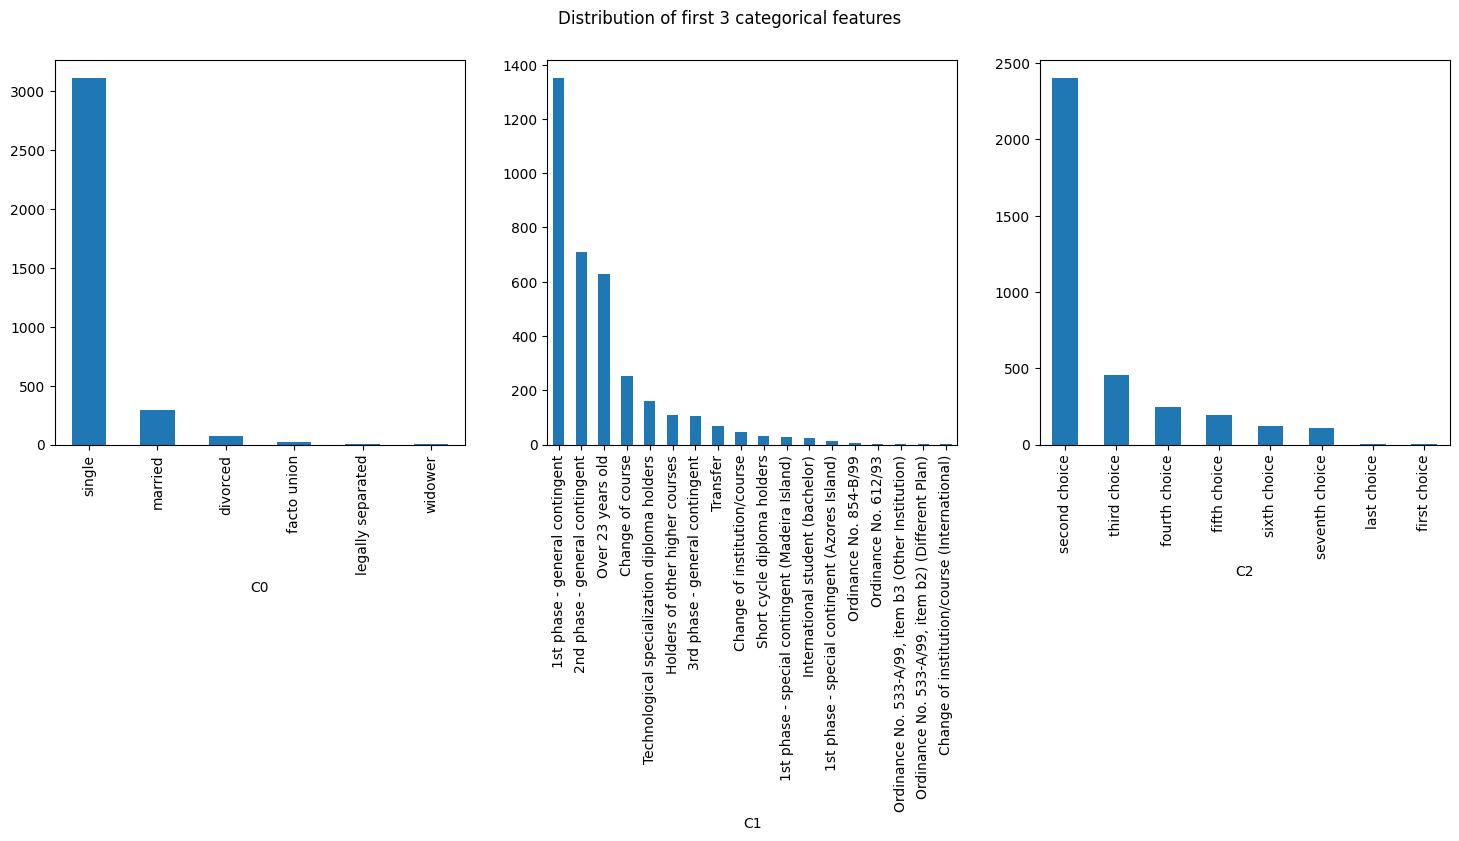
\includegraphics[width=\textwidth]{figures/q3_categorical_distribution.png}
			\caption{Distribution of the first 3 categorical features}
			\label{}
		\end{figure}

	\item \textbf{[Q4] Outliers}
		\begin{itemize}
			\item \textbf{Detection}: 

				The first detection method I used is to identify values that are more than 1.5 times the interquartile range away from mean. For C6, C14, C15, I identify 77+70, 0+340, 0+454 potential outliers respectively. (In A+B, A indicates the number of outliers smaller than mean minus 1.5 times iqr while the number of outliers is larger than the mean plus 1.5 times iqr).

				(Part of) outliers identified for C6, C14, C15 (from left to right)
				\begin{center}
					\begin{tabular}{|c|c|}
						\hline
						instance id & value \\
						\hline
						18      & 50.0 \\
						20      & 50.0 \\
						114     & 50.0 \\
						307     & 50.0 \\
						387     & 50.0 \\
						... & \\ 
						3236    & 50.0 \\
						3317    & 50.0 \\
						3370    & 50.0 \\
						3431    & 50.0 \\
						3536    & 50.0 \\

						59      & 88.5 \\
						77      & 84.0 \\
						93      & 84.0 \\
						101     & 85.0 \\
						171     & 86.0 \\
						...     & \\
						3332    & 82.5 \\
						3373    & 95.0 \\
						3427    & 82.0 \\
						3487    & 90.0 \\ 
						3490    & 88.5 \\
						\hline
					\end{tabular}
					\hfill
					\begin{tabular}{|c|c|}
						\hline
						instance id & value \\
						\hline
						0       & 35 \\
						3       & 42 \\
						40      & 35 \\
						47      & 38 \\
						49      & 42 \\
						\ldots  & \ldots \\
						3463    & 41 \\
						3484    & 38 \\
						3499    & 37 \\
						3518    & 36 \\
						3523    & 37 \\
						\hline

					\end{tabular}
					\hfill
					\begin{tabular}{|c|c|}
						\hline
						instance id & value \\
						\hline
						5       & 2 \\
						12      & 2 \\
						14      & 1 \\
						17      & 3 \\
						18      & 11 \\
						\ldots & \ldots\\
						3499    & 5 \\
						3500    & 11 \\
						3512    & 7 \\
						3528    & 8 \\
						3534    & 1 \\
						\hline
					\end{tabular}
				\end{center}
				In the above table, outlier with abnormally small value is listed first (such outliers only exist for C6), followed by abnormally large values.

				The second detection method I used is \texttt{IsolationForest(contamin\-ation=0.1)}. Using this, I identified 341, 340, and 325 outliers in C6, C14, and C15 respectively.

				(Part of) outliers identified for C6, C14, C15 (from left to right)
				\begin{center}
					\begin{tabular}{|c|c|}
						\hline
						instance id & value \\
						\hline
						18    & 50.0 \\
						20    & 50.0 \\
						41    & 80.5 \\
						52    & 55.5 \\
						59    & 88.5 \\
						...   & ... \\
						3450  & 53.5 \\
						3469  & 80.5 \\
						3487  & 90.0 \\
						3490  & 88.5 \\
						3536  & 50.0 \\
						\hline
					\end{tabular}
					\begin{tabular}{|c|c|}
						\hline
						instance id & value \\
						\hline
						0      & 35 \\
						3      & 42 \\
						40     & 35 \\
						47     & 38 \\
						49     & 42 \\
						...    & ... \\
						3463   & 41 \\
						3484   & 38 \\
						3499   & 37 \\
						3518   & 36 \\
						3523   & 37 \\
						\hline
					\end{tabular}
					\begin{tabular}{|c|c|}
						\hline
						instance id & value \\
						\hline
						14     & 1  \\
						18     & 11 \\ 
						33     & 8  \\
						48     & 5  \\
						58     & 7  \\
						...    & ...\\
						3499   & 5  \\
						3500   & 11 \\
						3512   & 7  \\
						3528   & 8  \\
						3534   & 1  \\
						\hline
					\end{tabular}
				\end{center}

			\item \textbf{Consideration}: Outliers could possibly be human errors in outputting the data. Hence, we may need to remove or replace them by imputation during preprocessing so that our model will not be biased. During modeling, we may also try both including and excluding the outliers to see which model gives a better performance.
		\end{itemize}

	\item \textbf{[Q5] Correlation Analysis}
		\begin{itemize}
			\item \textbf{Feature Correlation} 

				The heatmap is visualized below:

				\begin{figure}[H]
					\centering
					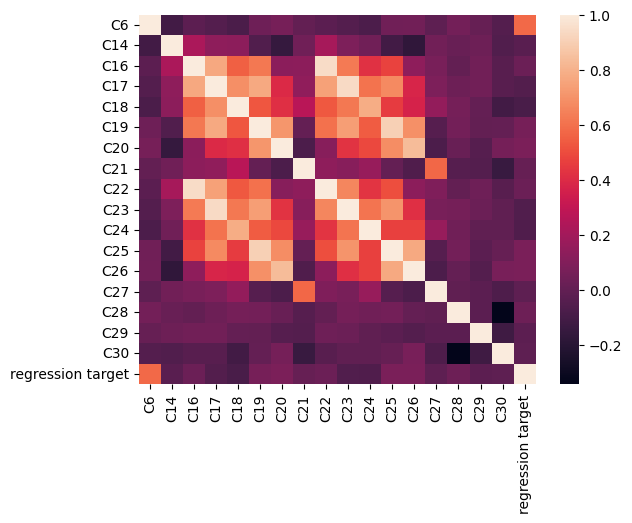
\includegraphics[width=0.8\textwidth]{figures/q5_heatmap.png}
					\caption{Correlation between every two features}
					\label{q5}
				\end{figure}
				
			\item \textbf{Insights}

				There is a lighter zone in between C16-C26, indicating these features have high correlation. We may limit our model to these features to simplify the architecture of neural network to obtain a better accuracy. Also, we may perform feature engineering to combine these features with \texttt{Polynomialfeatures()} to enhance the expressibility of the model. For example, we can add a column containing the element-wise multiplication of C22 and C17 since their correlation is quite high.
		\end{itemize}

	\item \textbf{[Q6] Initial Thoughts on Preprocessing}
		\begin{itemize}
			\item First, since there are missing values, we'll need to perform imputation on both numerical and categorical features. Then, we need to perform standardization on numerical features since each feature contains data with varying range. Furthermore, we need to perform encoding of categorical variables. Finally, we can select feature selection and feature engineering.
			\item Outlier detection and handling, imputation of missing values, feature selection and engineering are best performed during preprocessing rather than model training.
		\end{itemize}

	\section*{Part 2: Data Preprocessing Techniques}
\item \textbf{[Q7] Handling Missing Values}: Taking numerical feature C17 as an example, before imputation, its distribution is as follows:
	\begin{center}
		\begin{tabular}{|c|c|}
			\hline
			count & 3391 \\
			mean & 6.242996 \\
			std & 2.475471 \\
			min & 0 \\
			25\% & 5 \\
			50\% & 6 \\
			75\% & 7 \\
			max & 26 \\
			\hline
		\end{tabular}
	\end{center}
	We can use either constant, mean, median, or mode on numerical features for imputation, we get three results (from left to right: constant, mean, median, mode)
	\begin{center}
		\begin{tabular}{|c|c|}
			\hline
			count & 3539 \\
			mean & 5.98 \\
			std & 2.72 \\
			min & 0 \\
			25\% & 5 \\
			50\% & 6 \\
			75\% & 7 \\
			max & 26 \\
			\hline
		\end{tabular}
		\begin{tabular}{|c|c|}
			\hline
			count & 3539 \\
			mean & 6.24 \\
			std & 2.42 \\
			min & 0 \\
			25\% & 5 \\
			50\% & 6 \\
			75\% & 7 \\
			max & 26 \\
			\hline
		\end{tabular}
		\begin{tabular}{|c|c|}
			\hline
			count & 3539\\
			mean & 6.23 \\
			std & 2.42 \\
			min & 0 \\
			25\% & 5 \\
			50\% & 6 \\
			75\% & 7 \\
			max & 26 \\
			\hline
		\end{tabular}
		\begin{tabular}{|c|c|}
			\hline
			count & 3539 \\
			mean & 6.23 \\
			std & 2.42 \\
			min & 0 \\
			25\% & 5 \\
			50\% & 6 \\
			75\% & 7 \\
			max & 26 \\
			\hline
		\end{tabular}
	\end{center}
	The zero imputation strategy is not adoptable since it drastically change the mean and increases the std after adding more data value, distorting the data distribution.	

	I see that all other imputation strategy decreases the standard deviation of distribution, which is normal since number of data increases. However, the mean strategy can preserves the mean of the original distribution. Yet this may not always be good since the mean is sensitive to outliers and may not be a good indicator of distribution. If there are many outliers in a feature column, median should be preferred over mean and mode since mean is sensitive to outlier and mode is not an accurate measure of central tendency for numerical data.
	
	For categorical feature, we can use \texttt{SimpleImputer()} with 'most-frequent' strategy since this is the only strategy that's available for categorical data. It will make the feature distribution more concentrated on frequent values.

	To summarise, we should use median strategy for numerical feature columns with outliers and most-frequent strategy for categorical feature columns

\item \textbf{[Q8] Normalization and Standardization}

	Using \texttt{StandardScalar()}, we have the following result:

	The first numerical feature column C6 before processing:
	\begin{center}
		\begin{tabular}{|c|c|}
			\hline
			0    & 65.00 \\
			1    & 65.00 \\
			2    & 59.50 \\
			3    & 66.55 \\
			4    & 71.00 \\
			5    & 70.00 \\
			6    & 57.50 \\
			7    & 65.50 \\
			8    & 70.00 \\
			9    & 80.00 \\
			\hline
		\end{tabular}
	\end{center}
		The first numerical feature column C6 after processing:
		\begin{center}
			\begin{tabular}{|c|c|}
				\hline
				0   & -0.200135 \\
				1   & -0.200135 \\
				2   & -1.031074 \\
				3   &  0.034039 \\
				4   &  0.706344 \\
				5   &  0.555264 \\
				6   & -1.333234 \\
				7   & -0.124595 \\
				8   &  0.555264 \\
				9   &  2.066063 \\
				\hline
			\end{tabular}
		\end{center}

		The feature distribution will be shifted to zero mean and unit variance. The main difference between \texttt{StandardScalar()}, \texttt{MinMaxScalar} and \texttt{Robust scalar} lie in how they normalize features. \texttt{StandardScalar()} assumes that the data follow the guassian distribution and transforms the values to zero mean and unit variance. \texttt{MinMaxScalar} scales the values to a specific range and does not assume any distribution in the original data. \texttt{RobustScalar()} removes the median and scale the data according to the inter-quartile range. This approach is more robust to outlier since inter-quartile range is used.

		To summarize, \texttt{StandardScalar()} can be used when the data follows a guassian distribution, \texttt{MinMaxScalar()} can be used when the data does not follow a guassian distribution, and \texttt{RobustScalar()} can be used when outliers affect the model performance.
	\item \textbf{[Q9] Encoding Categorical Variables} \\
		Using \texttt{OneHotEncoder()}, we obtain the following result on C0.

		The first categorical feature C0 before processing:

		\begin{center}
			\begin{tabular}{|c|c|}
				\hline
				0    &  divorced \\
				1    &  single \\
				2    &  single \\
				3    &  married \\
				4    &  single \\
				5    &  single \\
				6    &  single \\
				7    &  single \\
				8    &  single \\
				9    &  single \\
				\hline
			\end{tabular}
		\end{center}
		
		The first categorical feature C0 after processing:

		\begin{center}
			\begin{tabular}{|c|c|c|c|c|c|}
				\hline
				& facto union  & legally separated & married & single & widower \\
				\hline
				0               & 0.0                  & 0.0        &  0.0        & 0.0        & 0.0 \\
				1               & 0.0                  & 0.0        &  0.0        & 1.0        & 0.0 \\
				2               & 0.0                  & 0.0        &  0.0        & 1.0        & 0.0 \\
				3               & 0.0                  & 0.0        &  1.0        & 0.0        & 0.0 \\
				4               & 0.0                  & 0.0        &  0.0        & 1.0        & 0.0 \\
				...             & ...                  & ...        &  ...        & ...        & ... \\
				3534            & 0.0                  & 0.0        &  0.0        & 1.0        & 0.0 \\
				3535            & 0.0                  & 0.0        &  0.0        & 1.0        & 0.0 \\
				3536            & 0.0                  & 0.0        &  0.0        & 1.0        & 0.0 \\
				3537            & 0.0                  & 0.0        &  0.0        & 1.0        & 0.0 \\
				3538            & 0.0                  & 0.0        &  0.0        & 1.0        & 0.0 \\	
				\hline
			\end{tabular}
		\end{center}

		Ordinal encoding should be used when we need to preserve the order of data, i.e. nominal data. For example, "first choice" can be encoded to 1, "second choice" can be encoded to 2, etc. One hot encoding should be used when the data do not have an inherent ordering, hence they should carry equal weighting.

	\item \textbf{[Q10] Feature Selection}

	Using \texttt{VarianceThreshold(threshold=0.01)} on numerical features, the following features are dropped:
	\begin{verbatim}
		['C0_legally separated', 'C0_widower',
		'C1_Change of institution/course (International)',
		'C1_Ordinance No. 533-A/99, item b2) (Different Plan)',
		'C1_Ordinance No. 533-A/99, item b3 (Other Institution)',
		'C1_Ordinance No. 612/93', 'C7_Colombian', 'C7_Cuban', 
		'C7_Dutch', 'C7_German', 'C7_Italian', 'C7_Lithuanian', 
		'C7_Mexican', 'C7_Moldova (Republic of)', 'C7_Mozambican', 
		'C7_Russian', 'C7_Turkish', 'C7_Ukrainian']
	\end{verbatim}
	because the variance in the feature column is too small to contribute anything reasonable to regression or classification. We see that most of them are one-hot encoded columns with very unbalanced value (i.e., most of them are 1s/0s)

	Using \texttt{SelectKBest(f\_classif, k=50)}, scikit-learn performs a one-way ANOVA test to find features that has a higher correlation with the target. For regression target, we drop the following:

	\begin{verbatim}
		['C28', 'C0_facto union', 'C0_legally separated', 
		'C0_widower', 'C1_1st phase - special contingent 
		(Azores Island)', 'C1_Change of institution/course',
		'C1_Change of institution/course (International)',
		'C1_International student (bachelor)',
		'C1_Ordinance No. 533-A/99, item b2) (Different Plan)',
		'C1_Ordinance No. 533-A/99, item b3 (Other Institution)',
		'C1_Ordinance No. 612/93', 'C1_Ordinance No. 854-B/99',
		'C1_Technological specialization diploma holders',
		'C3_Journalism and Communication', 'C3_Oral Hygiene',
		'C3_Social Service (evening attendance)', 'C7_Brazilian',
		'C7_Cape Verdean', 'C7_Colombian', 'C7_Cuban', 
		'C7_Dutch', 'C7_German', 'C7_Guinean', 'C7_Italian', 
		'C7_Mexican', 'C7_Moldova (Republic of)', 'C7_Mozambican', 
		'C7_Portuguese', 'C7_Spanish', 'C7_Turkish', 'C7_Ukrainian', 
		'C9_yes', 'C15_yes']
	\end{verbatim}

	For classification target, we drop the following:

	\begin{verbatim}
		['C16', 'C21', 'C22', 'C27', 'C29', 'C30', 
		'C0_facto union', 'C0_legally separated', 
		'C0_widower', 'C1_Change of course',
		'C1_Change of institution/course',
		'C1_Change of institution/course (International)',
		'C1_International student (bachelor)',
		'C1_Ordinance No. 533-A/99, item b2) (Different Plan)',
		'C1_Ordinance No. 533-A/99, item b3 (Other Institution)',
		'C1_Ordinance No. 612/93', 
		'C1_Short cycle diploma holders',
		'C1_Transfer', 'C3_Equinculture', 'C3_Management',
		'C3_Management (evening attendance)', 'C7_Colombian', 
		'C7_German', 'C7_Guinean', 'C7_Italian', 'C7_Lithuanian', 
		'C7_Moldova (Republic of)', 'C7_Mozambican', 'C7_Russian', 
		  'C7_Santomean', 'C7_Spanish','C7_Turkish', 'C2_ordinal'],
	\end{verbatim}

	  These feature have a low correlation with the target and thus may hinder the model's ability for classification/regression.

	\item \textbf{[Q11] Feature Engineering}:
		We can use polynomial features engineering on features having a high correlation with the target values (e.g., those selected by \texttt{SelectKBest()}). For example, from Q5, we know that C22 and C16 have high correlation value, we can add a column C22 * C16. This provides the model with ability to classify the data with a non-linear boundary (with respect to the original degree 1 values). Hence, the model can learn better the relationship between features and targets.

		\section*{Part 3 Regression}
		\subsection*{Linear Regression}
	\item \textbf{[Q12]} By running select k best with k=6, we found that the best six features are [C6, C1\_Ordinance No. 854-B/99, C7\_Cape Verdean, C7\_Cuban, C7\_Mexican, C7\_Ukrainian]. Running regression on them produce the following result:
		\begin{center}
			\begin{tabular}{|c|c|c|}
				\hline
				Feature & $R^2$ score & Mean Squared Error \\
				\hline
				C6 & 0.3457983 & 0.003182307610 \\
				C1\_Ordinance No. 854-B/99 & 0.011548403 & 0.0048082 \\
				C7\_Cape Verdean & 6.996831e-05 & 0.004864073 \\
				C7\_Cuban & -0.0005831622 & 0.004867250 \\
				C7\_Mexican & -0.0005571542 & 0.004867124 \\
				C7\_Ukrainian & 0.004605998 & 0.004842008 \\
				\hline
			\end{tabular}
		\end{center}
		training with all 6 features yield an $R^2$ score of $0.348$ and mean squared error of $0.00484$.
	\item \textbf{[Q13]} From the above table, a better $R^2$ score also has a lower mean squared error rate. Hence, they are correlated.
	\item \textbf{[Q14]} For a binary categorical variable, they are encoded with either $1$ or $0$.  Categories that are encoded with $0$ do not affect model output while categories encoded with $1$ may either get a negative or positive weight, indicating a negative or positive relationship with regression target, respectively.
	Using the C2 ordinal variable (which has 7 possible values, encoded ordinally) for regression, we obtain an $R^2$ score of $0.00244$ and mean squared error of $0.00485$
		\subsection*{Feedforward Neural Networks}
	\item \textbf{[Q15]}
		The model setting is an MLP regressor with three layers of hidden neurons of $h$ units, with \texttt{early\_stopping = true}. Time is in second in the following table.
		\begin{center}
			\begin{tabular}{|c|c|c|c|c|}
				\hline
				h & time (mean) & time (std) & $R^2$ score (mean) & $R^2$ score (std) \\
				\hline
				1 & 2.21 & 0.84 & -0.001 & 0 \\
				8 & 0.73 & 0.22 & 0.37 & 0 \\
				32 & 1.14 & 0.004 & 0.379 & 0 \\
				128 & 1.65 & 0.324 & 0.384 & 0 \\
				\hline
			\end{tabular}
		\end{center}
		\begin{figure}[H]
			\centering
			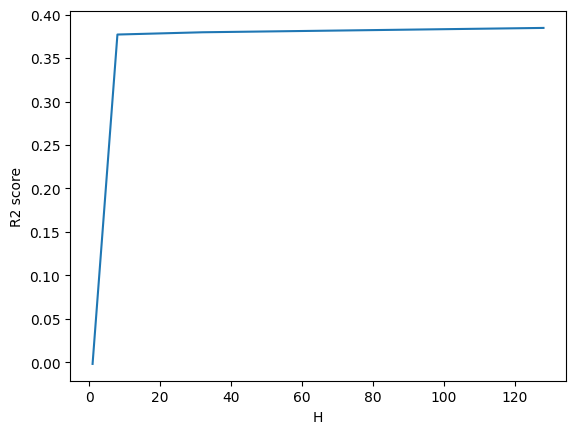
\includegraphics[width=0.8\textwidth]{figures/q15_r2_score.png}
			\caption{$R^2$ score against number of neurons}
			\label{q15}
		\end{figure}
	\item  \textbf{[Q16]} The training time for linear regression model is 0.01s. The best MLP model with $h=32$ is slower than linear regression model by 164 times. The $R^2$ score of MLP model is better than the linear regression model by $0.384-0.00484 = 0.38$.

	\item \textbf{[Q17]} For classification, we apply variance threshold of 0.1 in [Q10]. The model setting log loss and optimal learning rate. We obtain the following result by changing the penalty in 
		\begin{verbatim}
			=========
			Elasticnet
			Mean accuracy:  0.8055555555555557 std:  0.029273618750865937
			Time: 0.11378812789916992 std:  0.003529139817117777
			F1 score: 0.8526807256827041 std:  0.03444454424581645
			=========
			l2
			Mean accuracy:  0.8681732580037664 std:  0.007678675343832401
			Time: 0.08564352989196777 std:  0.011466927441279712
			F1 score: 0.9073794416512456 std:  0.008758999930354084
			=========
			l1
			Mean accuracy:  0.8427495291902072 std:  0.01640419151618109
			Time: 0.10757311185201009 std:  0.004443627139115725
			F1 score: 0.8799707892351479 std:  0.015349040241937445
			=========
		\end{verbatim}
	\item \textbf{[Q18]}
		\begin{figure}[H]
			\centering
			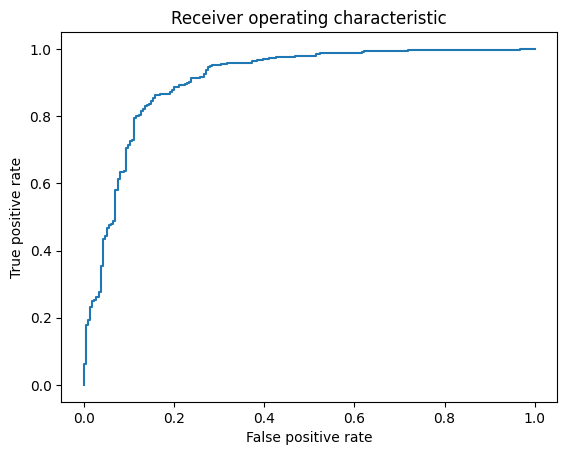
\includegraphics[width=0.8\textwidth]{figures/q18_roc_curve.png}
			\caption{ROC curve for the l1 model}
			\label{roc_curve}
		\end{figure}
		The AUC value is 0.9066 for the last model. We need to examine the ROC curve since it tells us the model performance of different classification threshold.
	\item \textbf{[Q19]} Using 'l1' penalty, the accuracy of different learning rate is given below:
		\begin{verbatim}
			=========
			eta:  0.01
			accuracy 0.8601694915254238
			f1_score 0.898876404494382
			=========
			eta:  0.05
			accuracy 0.8615819209039548
			f1_score 0.9006085192697768
			=========
			eta:  0.1
			accuracy 0.8968926553672316
			f1_score 0.9301435406698565
			=========
			eta:  0.15
			accuracy 0.8757062146892656
			f1_score 0.9185185185185185
			=========
			eta:  0.2
			accuracy 0.8220338983050848
			f1_score 0.8668076109936576
			=========
			eta:  0.25
			accuracy 0.8234463276836158
			f1_score 0.8715313463514903
			=========
			eta:  0.3
			accuracy 0.8248587570621468
			f1_score 0.870020964360587
			=========
		\end{verbatim}
		\subsection{Feedforward Neural Network}
	\item \textbf{[Q20]} The model setting is the default \texttt{MLPClassifier()} setting with \texttt{early stopping = True}. The model accuracy and time is presented below
		\begin{center}
			\begin{tabular}{|c|c|c|c|c|}
				\hline
				h & time (mean) & time (std) & accuracy (mean) & accuracy (std) \\
				\hline
				1 & 0.30 & 0.0208 & 0.30 & 0 \\
				8 & 1.18 & 0.36 & 0.88 & 0 \\
				32 & 0.773 & 0.334 & 0.880 & 0 \\
				128 & 1.32 & 0.019 & 0.87 & 0 \\
				\hline
			\end{tabular}
			\vspace{1cm}
			\begin{tabular}{|c|c|c|}
				\hline
				h & $F1$ score (mean) & $F1$ score (std) \\
				\hline
				1 & 0 & 0 \\
				8 & 0.92 & 0 \\
				32 & 0.91 & 0 \\
				128 & 0.91 & 0\\
				\hline
			\end{tabular}
		\end{center}

	\item \textbf{[Q21]} A possible reason for the difference in F1 score and accuracy is because of imbalance of TP, TN, FP, and FN. F1 score is given by $\frac{2TP}{2TP+FP+FN}$ and accuracy is given by $\frac{TP+TN}{TP+TN+FP+FN}$. If the majority of classification belongs to TP (e.g., TP=1, TN=0, FP=1, FN=0), F1-score will be higher than accuracy as in our model.
		\begin{figure}[H]
			\centering
			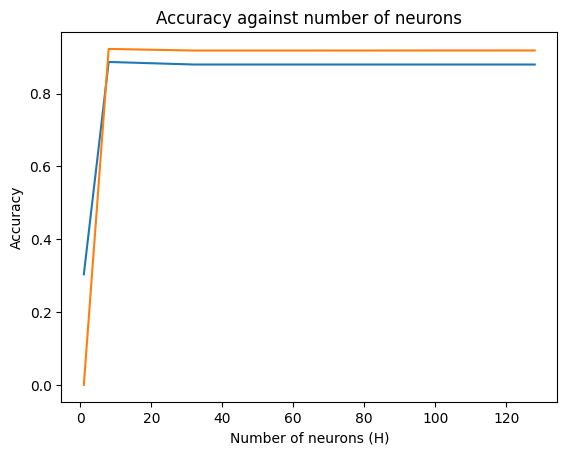
\includegraphics[width=0.8\textwidth]{figures/q21_accuracy.png}
			\caption{Accuracy (in blue) and F1-score (in orange) against number of neurons}
			\label{q20}
		\end{figure}
	\item \textbf{[Q22]} The training time of neural network is about 10 times that of a logistic regression model. The accuracy and f1-score of neural network is about the same as the logistic regression model, both having 0.88 accuracy and 0.93 f1-score.

	\item \textbf{[Q23]} The accuracy increases when H increases from 1 to 8 but slightly drop when H increases more from 8 to 128. The initial jump is due to the non-linearity introduced by MLP while the dip can be explained by possible overfitting or the MLP is stuck in some local minimum during gradient descent.

	\item \textbf{[Q24], [Q25], [Q26]} Combination A, B, C give an accuracy of 0.884, 0.874, and 0.901 respectively, while the f1-scores are 0.918, 0.913, and 0.932 respectively.

	\item \textbf{[Q27]} We tried the following 5 combinations:
		\begin{verbatim}
		pipe_parameters = [
			{
			  'classifier__batch_size': [16, 32, 64, 128, 256]
			}
		]	
		\end{verbatim}

		The result of the five combination is as followed: 
		\begin{center}
			\begin{tabular} {|c|c|c|c|c|c|}
				\hline
				mean accuracy & 0.8685 & 0.8721 & 0.8668 & 0.8728 & 0.868 \\
				std accuracy & 0.0203 & 0.0160 & 0.0181 & 0.0189 & 0.0197 \\
				\hline
			\end{tabular}
		\end{center}
		The accuracy is the best when the batch-size is 128 with constant learning rate, with an accuracy of 0.872. Although the accuracy is lower than that of Q26, this may be due to different split of the train test dataset.
\end{description}

\end{document}
